\section{The End-to-End System}\label{sec:system}

UniPlan is a web application (\texttt{python3 main.py}). A student adds units and writes one sentence. The page writes what it read beside each clause and turns unsure clauses into two-option questions (Figure~\ref{fig:app}). Only after the student accepts or corrects these notes does the scheduler run. The student then sees three weekly grids with one-line reasons, can switch to all the distinct options kept, and can download a calendar file.

\begin{figure}[h]
	\centering
	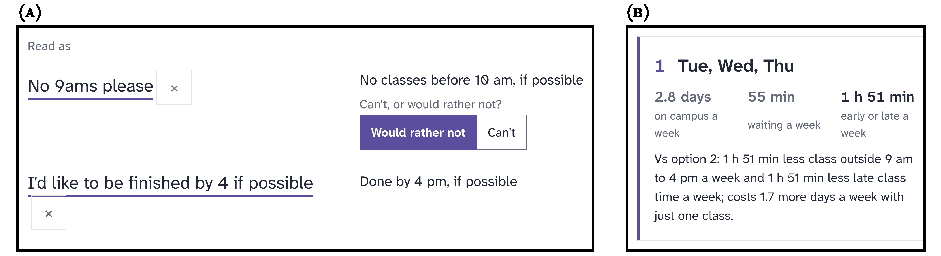
\includegraphics[width=\textwidth]{figures/fig_app.pdf}
	\caption{The web page with the deployed models on exam item e121 (AI-written). (a)~``No 9ams'' was read as a preference, so the page asks. (b)~After ``Can't'', the first of three picks with its reason.}
	\label{fig:app}
\end{figure}

Each AI output has a limited job. Parsed conditions are a draft that becomes binding only after the student confirms it; the ranking decides which timetables are shown first, never which exist; and the reasons come from the ranker's own contributions and are checked against the timetable. This follows the mixed-initiative pattern of the Week~7 lecture, where the AI points out missing constraints and the person decides~\cite{engg2112_w07}. The system also degrades gracefully: if the GPU server does not answer, it uses the model on the local machine and then, within 15~s, the TF-IDF classifier (\pRtwoC\% to \pLinC\% of clauses right on the exam), and asks the student to check each condition; if nothing fits, it names the clashing activities and offers the closest timetables with each broken limit stated.

\textbf{Deployment.} The run-time code uses only the Python standard library, and the fine-tuned model runs in Ollama on a single GPU. With the parser on one laptop GPU over the local network, a sentence for two to four units takes about \plMedianRec{}~s end to end, so one GPU server could serve many students, but enrolment opens for everyone at once and would need queueing; we did not load-test this. A real deployment would also need an official timetable feed or written permission from the university, seat numbers refreshed near enrolment day, and a pilot with real students (Section~\ref{sec:recs}).
